\documentclass[dvipdfmx]{standalone}

\usepackage{tikz}

\begin{document}
\begin{tikzpicture}
    \node[anchor=west] at (-1,3) {105円分の支払いが100円未満の硬貨でされたならば、};

    \node at (0,2) {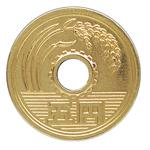
\includegraphics[width=1cm]{../imgs/yen/5.jpg}};
    \node at (1,2) {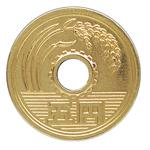
\includegraphics[width=1cm]{../imgs/yen/5.jpg}};
    \node at (2,2) {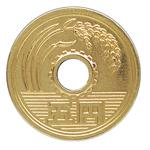
\includegraphics[width=1cm]{../imgs/yen/5.jpg}};
    \node at (3,2) {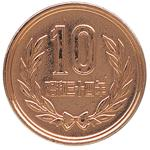
\includegraphics[width=1cm]{../imgs/yen/10.jpg}};
    \node at (4,2) {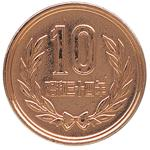
\includegraphics[width=1cm]{../imgs/yen/10.jpg}};
    \node at (5,2) {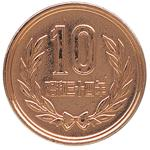
\includegraphics[width=1cm]{../imgs/yen/10.jpg}};
    \node at (6,2) {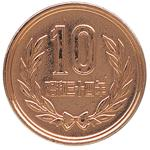
\includegraphics[width=1cm]{../imgs/yen/10.jpg}};
    \node at (7,2) {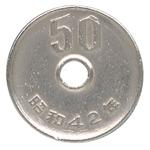
\includegraphics[width=1cm]{../imgs/yen/50.jpg}};

    \node[anchor=west] at (-1,1) {5円硬貨3枚などの無駄が存在する。};

    \node at (0,0) {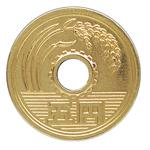
\includegraphics[width=1cm]{../imgs/yen/5.jpg}};
    \node at (1,0) {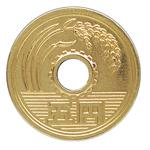
\includegraphics[width=1cm]{../imgs/yen/5.jpg}};
    \node at (2,0) {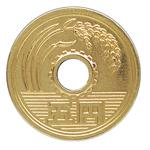
\includegraphics[width=1cm]{../imgs/yen/5.jpg}};
    \node at (3,0) {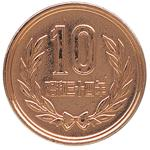
\includegraphics[width=1cm]{../imgs/yen/10.jpg}};
    \node at (4,0) {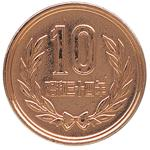
\includegraphics[width=1cm]{../imgs/yen/10.jpg}};
    \node at (5,0) {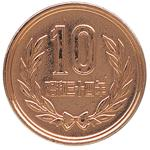
\includegraphics[width=1cm]{../imgs/yen/10.jpg}};
    \node at (6,0) {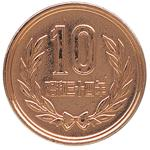
\includegraphics[width=1cm]{../imgs/yen/10.jpg}};
    \node at (7,0) {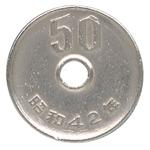
\includegraphics[width=1cm]{../imgs/yen/50.jpg}};

    \draw[very thick,red] (-0.5,0.5) rectangle (2.5,-0.5);

    \node[anchor=west] at (-1,-1) {あるいは、100円分ちょうどを選べる。};

    \node at (0,-2) {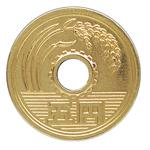
\includegraphics[width=1cm]{../imgs/yen/5.jpg}};
    \node at (1,-2) {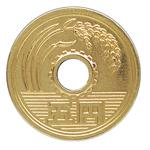
\includegraphics[width=1cm]{../imgs/yen/5.jpg}};
    \node at (2,-2) {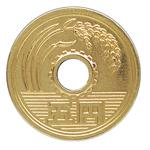
\includegraphics[width=1cm]{../imgs/yen/5.jpg}};
    \node at (3,-2) {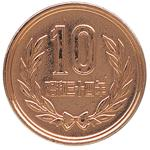
\includegraphics[width=1cm]{../imgs/yen/10.jpg}};
    \node at (4,-2) {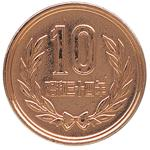
\includegraphics[width=1cm]{../imgs/yen/10.jpg}};
    \node at (5,-2) {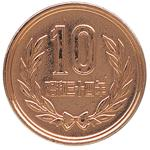
\includegraphics[width=1cm]{../imgs/yen/10.jpg}};
    \node at (6,-2) {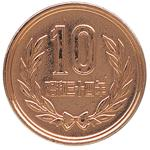
\includegraphics[width=1cm]{../imgs/yen/10.jpg}};
    \node at (7,-2) {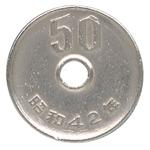
\includegraphics[width=1cm]{../imgs/yen/50.jpg}};

    \draw[very thick,red] (0.5,-1.5) rectangle (7.5,-2.5);
\end{tikzpicture}
\end{document}
